% Chapter 1

\chapter{Introduction} % Chapter title

\label{ch:introduction} % For referencing the chapter elsewhere, use \autoref{ch:introduction} 

%----------------------------------------------------------------------------------------

Building and analyzing a proposition store for emotion detection

Emotion detection can be considered a subtask of sentiment analysis.
Sentiment analysis is the study of analyzing a person's opinion or mental state of mind concerning a certain topic or concept. It has been used in a wide array of commercial and non-commercial applications, such as sentiment mining, etc. While sentiment analysis is mainly concerned with identifying positive or negative opinons towards concepts, emotion detection deals with detecting emotions in text.

The binary classification of sentiment analysis falls short in light of the variety and multifacetedness of human sentiment and emotion.
Sentiment is one of the primary factors that make us human.\\

To avoid ambiguity, we will conceive of sentiment in the following as being differentiated in positive, negative, and neutral, whereas we define emotion as being more varied, encompassing emotions such as anger, hate, etc.\\

As becomes clear, emotion (in contrast to sentiment) is not clearly defined. Humans are able to express a panoply of emotions. A clear classification, though, is anything but obvious. Emotions have been abundantly studied in psychology. Different models have been proposed trying to represent and model the relationship of emotions. (comparison)

We will make use of one of the most pervasive ones that has been used in different applications.

Plutchik's emotion model classifies emotions in eight base groups: anger, anticipation, disgust, fear, joy, sadness, surprise, and trust. We will take these as the basic emotions that we use for our classification.

As a sentiment analysis task, emotion detection has been implemented using machine learning or lexicon-based approaches, although lexicon-based approaches have been used more frequently.

\citeauthor{sentiment_analysis_association_metrics}


\begin{figure}[bth]
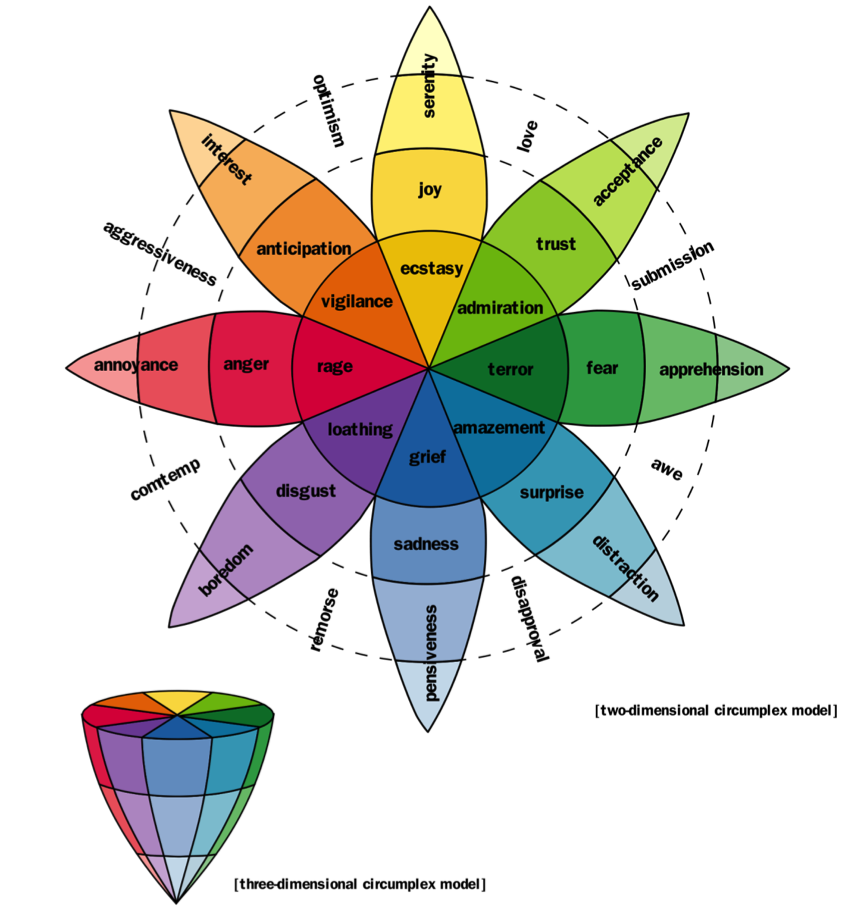
\includegraphics[width=.80\linewidth]{gfx/plutchik_wheel_emotion.png}
\caption{Plutchik's emotion whell}\label{fig:plutchik}
\end{figure}

The use of sentiment lexica has a long history in sentiment analysis. Beginning with the General Inquirer which initially contained a psycho-sociological dictionary and was used e.g. to differentiate fake suicide notes from real ones. \cite{stone_al_general_inquirer}



As sentiment lexica have been excessively used for the purposes of sentiment analyses, we will build one for emotion detection and show how it can be used in different applications.

The manual compilation of a sentiment lexicon can be a long and tedious process. Recently, researchers have looked for other methods for building a sentiment lexicon: 
\citeauthor{mohammad_crowdsource_sentiment_lexicon} used crowd-funding to build an emotion lexicon.

Not only differentiating emotions but also identifying the perspective and the target of the emotion proves to be challenging. \citeauthor{das_emotion_holder} use VerbNet frames to identify the emotion holder.

We use the Annotated Gigaword API \cite{napoles_al_annotated_gigaword}.

First we compile patterns that we use for extraction. We evaluate these and then we use them for extraction from the annotated Gigaword corpus. Later we analyse the extractions and evaluate whether they are associated with the respective emotions. Finally, we explore how they can be used to enable different applications of emotion analysis.



Inspiration from Emotion holder paper
In psychology and common use, emotion is an aspect of a person's mental state of
being, normally based in or tied to the person's internal (physical) and external (so-
cial) sensory feeling. The determination of emotion expressed in the text with
respect to reader or writer is itself a challenging issue. Emotion holder extraction
research is important for discriminating between emotions that are viewed from dif-
ferent perspectives. A wide range of Natural Language Processing (NLP) tasks
such as tracking users' emotion about products or events or about politics as ex-
pressed in online forums or news, to customer relationship management are using
emotional information. So, the determination of emotion holder from the text invokes
a challenge and helps us track and distinguish user's emotion separately.
In linguistics, a grammatical agent or holder is the participant of a situation that carries out the action and also, agent or holder is the name of the thematic role.
